\graphicspath{{chapters/images/0204/}}

\chapter{Generalized linear models}


\begin{definition} \label{def: RegModel} A regression model provides a function
  that describes the relationship between one or more independent variables and
  a response, dependent, or target variable (definition taken from
  \href{https://www.imsl.com/blog/what-is-regression-model}{Reference-Site}).
\end{definition}

  \textbf{Generalized linear models (GLMs)} are a broad family of regression
  models which includes, for instance, linear, logistic and poisson regressions
  (and many more, some of them are shown in figure \ref{fig: modelsregress}).
  The concept was created by Nelder and Wedderburn in 1972, in order to map into
  a single framework all regressions models. In general regression models are
  characterized by:
  \begin{itemize}
    \item $Y$: the random \textbf{response variable} you want to predict
    \item $\vec{X}=(X_1, \dots, X_p)$: a \textbf{vector of random predictors}
    (generally known)
  \end{itemize}
  Notice that, since these models describe the value of $Y$ with respect to the
  vector $\vec{X}$ (they give the value of $Y|\vec{X}=\vec{x}$), they do not
  give information on the actual distribution of $Y$, but rather on the values
  that it takes conditionally to the values taken by the predictors, which can
  be written as

  \begin{figure}[H]
    \caption{The values of a specific $Y_i$ are not distributed in the same way as the other $Y_i$ usually}
    \centering
    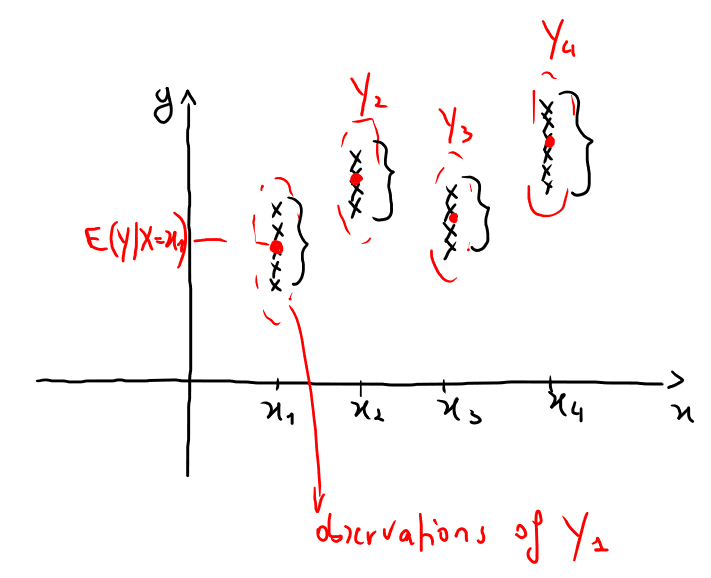
\includegraphics[width=0.5\textwidth]{GeneralizedLinModels}
    \label{fig: diffdistrib}
    \end{figure}

  $$Y_i=(Y|\vec{X}=\vec{x}_i)$$ Therefore, if you have $n$ vectors of random
  predictors, $Y_1, \dots, Y_n$ are independent random variables but generally
  they are not identically distributed, as shown in figure \ref{fig:
  diffdistrib}.
  %TODO Add images

  \section{From linear models to generalized linear models} \label{sect:
  GenLinModels}
  
  Linear models make some implicit assumptions that must be removed in order to
    generalize.
    
    \begin{tabularx}{1\textwidth}{>{\centering\arraybackslash}X
      >{\centering\arraybackslash}X }

    % \caption{dfidfidfi}\label{prova} \\
    % whould be useful to add caption #TODO


    \textbf{Linear models} & \textbf{Generalized linear models} \\

    $Y_i \sim N(\mu_i, \sigma^2)$ & $Y_i \sim f(y_i; \mu_i, \phi)$\\

    $\mu_i = E[Y_i] = E[Y|\vec{X} = \vec{x}_i] = \eta_i$ & $g(\mu_i) = \eta_i$
    \\

    $\eta_i = \vec{x}_i^t\vec{\beta} = \beta_0x_{i0} + \beta_1x_{i1} + \dots +
    \beta_px_{ip}$ & $\eta_i = \vec{x}_i^t\vec{\beta}$\\
    
    \end{tabularx}
\\
\\
    First of all, linear models assume that the each observation (random
    variable) $Y_i$ is normally distributed, with mean $\mu_i$, meaning that
    $E[Y|\vec{X}=\vec{x}_i] = \mu_i$, and $\sigma^2 = Var(Y_i) =
    Var(Y|\vec{X}=\vec{x}_i)$. It also assumes that the variance is constant,
    therefore \emph{homoskedasticity} is taken as a fundamental condition. The
    values of each mean $\mu_i$ is calculated exactly through this calculation:
    $\mu_i = x_i^t \beta = \nu_i$. The $\beta$ coefficients are calculated
    through tecniques like the Least Square method and the Maximum Likelihood
    Estimation.\\
    
    On the other hand, Generalized Linear Models do not make any assumptions on
    the shape of the distribution from which it comes $Y_i$:  \emph{$Y_i$ is
    distributed according to some function $f(y_i)$ with the parameters $\mu_i$
    and $\phi$}. $\phi$ is called \textbf{special parameter} and it may or may
    not be present in the model. The \textbf{linear predictor} is the function
    used to predict the outcome of the random variable $Y_i$ knowing some values
    for the predictor $\vec{X}_i$; in both cases the linear predictor is defined
    as $\eta_i = \vec{x}_i^t\vec{\beta} = \beta_0x_{i0} + \beta_1x_{i1} + \dots
    + \beta_px_{ip}$, where $p$ is the number of parameters and the coefficients
    $\beta_0, \dots, \beta_p$ are the weights for the predictors. \\
    \noindent In generalized linear models $\mu_i$ and $\eta_i$ are related by a
    \textbf{link function}, which is a function $g$ of $\mu_i$ such that
    $g(\mu_i) = \eta_i$. Contrarily to what we would think, the link function
    doesn't represent a tranformation \\
    
    A generalized linear model is then obtained by choosing
    \begin{itemize}
      \item The \textbf{systematic component}: represents the "correlation"
      between the predictors and the outcome \label{sent: linkFunc}
      \item The \textbf{link function}: a function that acts over the the
      systematic component, it "delinearizes" the correlation between predictors
      and outcomes.
      \item The \textbf{random component}: it is the distribution of the
      observations. They could be distributed in different ways, including
      Poisson, negative binomial excetera. \\
    \end{itemize}

    \noindent A \underline{linear regression model} is for example obtained
    considering:
    
    \begin{itemize}
      \item link function: 1, since systemic component ($\beta^t \vec{x}$)
      remains linear
      \item random component: normal distribution, since all $Y_i$ are normally
      distributed
    \end{itemize}
    
    % a distribution function $f$ and a link function $g$; for instance, if $f$
    % is a normal distribution (with $\sigma^2 = \phi$) and $g$ is the identity
    % function (therefore $\mu_i = \eta_i$), we get the linear model. 

    A series of possibly makable models are reported in the \ref{fig:
    modelsregress}.
  
    \begin{figure}[h]
      \caption{Here are represented for each line a type of regression model obtained as a generalized linear model}
      \centering
      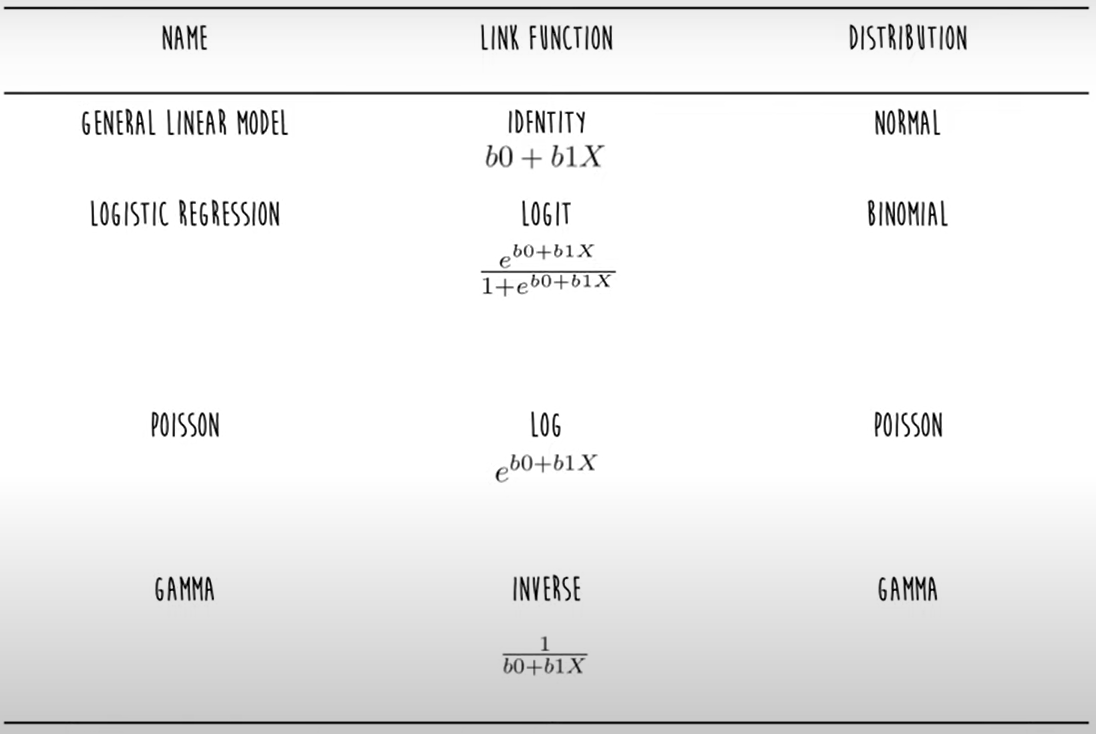
\includegraphics[width=0.55\textwidth]{ModelsWithDifferentCompositions}
      \label{fig: modelsregress}
      \end{figure}


  \section{Exponential dispersion family}
    The function $f$, describing the distribution of the random variable $Y_i$,
     needs to be a member of the \textbf{exponential dispersion family (EDF)}. A
     density belonging to the EDF can be written as

     \begin{equation} \label{eq: EDF}
      f(y_i;\theta_i,\phi)=\exp\left\{\frac{y_i\theta_i-b(\theta_i)}{a_i(\phi)}+c(y_i;\phi)\right\}
     \end{equation}

    where:
    \begin{itemize}
      \item $f(y_i, \theta_i, \phi)$ is the density function that has to be
      tested. $\theta_i$ and $\phi$ are some parameters. The values of
      $\theta_i$ are called \textit{canonical parameters}.
      \item $a_i$, $b$ and $c$ are some other functions.
    \end{itemize}
    
	It is obvious that, if a density function could be related to this family, it
	is possible to  derive from it the functions $a_i$, $b$ and $c$, and the
	parameter $\theta_i$. Now we'll try to understand if some important density
	functions belong to the EDF family.

    \subsection{Example: normal distribution is a member of the EDF}
      We want to demonstrate that the normal distribution is a member of the
      EDF.
      \begin{align*}
      f(y_i; \mu_i, \sigma^2)
        &= \frac{1}{\sqrt{2\pi\sigma^2}} \exp\left\{-\frac{1}{2} \frac{(y_i-\mu_i)^2}{\sigma^2}\right\}
        & \text{ definition of normal distribution}\\
        &= \exp\left\{-\frac{1}{2} \frac{(y_i-\mu_i)^2}{\sigma^2} + \log\left(\frac{1}{\sqrt{2\pi\sigma^2}}\right)\right\}
        & \text{ pull coefficient inside the exponential}\\
        &= \exp\left\{-\frac{1}{2} \frac{(y_i-\mu_i)^2}{\sigma^2} -\frac{1}{2}\log\left(2\pi\sigma^2\right)\right\}
        & \text{ rearrange using log properties}\\
        &= \exp\left\{-\frac{1}{2} \frac{y_i^2-2y_i\mu_i+\mu_i^2}{\sigma^2} -\frac{1}{2}\log\left(2\pi\sigma^2\right)\right\}
        & \text{ compute the square}\\
        &= \exp\left\{\frac{y_i\mu_i+\nicefrac{\mu_i^2}{2}}{\sigma^2} - \frac{1}{2\sigma^2}y_i^2 - \frac{1}{2}\log\left(2\pi\sigma^2\right)\right\}
        & \text{ group terms containing } \mu_i\\
      \end{align*}
      The normal distribution therefore belongs to the EDF by setting:
      \begin{align*}
        \theta_i     &= \mu_i, \\
        \phi         &= \sigma^2, \\
        b(\theta_i)  &= \nicefrac{\theta_i^2}{2}, \\
        a_i(\phi)    &= \phi, \\
        c(y_i; \phi) &= - \frac{1}{2\phi} y_i^2 - \frac{1}{2}\log(2\pi\phi)
      \end{align*}

    \subsection{Example: binomial distribution is a member of the EDF}
      We want to demonstrate that the binomial distribution is a member of the
      EDF.
      \begin{align*}
      f(y_i; n_i, \pi_i)
        &= \binom{n_i}{y_i}\pi_i^{y_i}(1-\pi_i)^{n_i-y_i}
        & \text{ definition of binomial distribution}\\
        &= \exp\,\left\{\log\left(\binom{n_i}{y_i}\pi_i^{y_i}(1-\pi_i)^{n_i-y_i}\right)\right\}
        & \text{ exponentiate to compare with EDF} \\
        &= \exp\,\left\{y_i\log\pi_i+(n_i-y_i)\log(1-\pi_i)+\log\binom{n_i}{y_i}\right\}
        & \text{ split log and simplify}\\
        &= \exp\,\left\{\frac{y_i\log\left(\frac{\pi_i}{1-\pi_i}\right)+n_i\log(1-\pi_i)}{1}+\log\binom{n_i}{y_i}\right\}
        & \text{ group terms containing } \pi_i
      \end{align*}

      The binomial distribution therefore belongs to the EDF by setting:
      \begin{align*}
        \theta_i     &= \log\left(\frac{\pi}{1-\pi}\right) \text{(\textbf{logit})} \\
        \phi         &= 1 \\
        b(\theta_i)  &= - n_i \log(1-\pi_i)\\
                     &= -n_i \log\left(1-\frac{e^{\theta_i}}{1 + e^{\theta_i}}\right) 
                     &&\text{substitution of } \pi_i \text{ because of the calculation in \ref{calc: pii}} \\
                     &= n_i \log\left(1 + e^{\theta_i}\right) \\
        a_i(\phi)    &= \phi \\ %Non capisco questo, non dovrebbe essere phi? #TODO
        c(y_i; \phi) &= \log\binom{n_i}{y_i}
      \end{align*}

We replaced  $\pi_i = \frac{e^{\theta_i}}{1 + e^{\theta_i}}$ since:

	\begin{align} \label{calc: pii}
	e^{\theta_i} &= \frac{\pi_i}{1-\pi_i} \\
  &\Rightarrow (1-\pi_i)e^{\theta_i} = \pi_i \notag\\ 
	&\Rightarrow e^{\theta_i} - \pi_i e^{\theta_i} = \pi_i \notag\\
  &\Rightarrow \pi_i = \frac{e^{\theta_i}}{1+ e^{\theta_i}} \notag
	\end{align}

      For the binomial distribution ($Y_i \sim Bin(n_i, \pi_i)$) it is possble
      to write the relation between $\theta_i$ to $\mu_i$.

      \begin{align*}
        E[Y_i] = \mu_i = n_i\pi_i = n_i\frac{e^{\theta_i}}{1 + e^{\theta_i}} && \text{Link between } \mu_i \text{ and } \theta_i  
      \end{align*}
      
      Consequently, it is possible to rewrite the value of $\theta_i$ as follows

      $$\pi_i = \frac{\mu_i}{n_i} \implies \theta_i =
      \log\left(\frac{\pi_i}{1-\pi_i}\right) =
      \log\left(\frac{\nicefrac{\mu_i}{n_i}}{1-\nicefrac{\mu_i}{n_i}}\right)=\log\left(\frac{\mu_i}{n_i-\mu_i}\right)$$
      Notice that \textbf{heteroskedasticity} in naturally embedded in the model
      since the variance depends on $\mu_i$:
      $$Var(Y_i) = n_i\pi_i(1-\pi_i) =
      n_i\frac{\mu_i}{n_i}\left(1-\frac{\mu_i}{n_i}\right) =
      \mu_i\left(\frac{n_i - \mu_i}{n_i}\right)$$ This hold true for all GLMs
      but linear models which is the only homoskedastic model of the group. Most
      datasets are not homoskedastic. 

      % \section{Connection between}
  \section{Connection between \texorpdfstring{$\theta_i$}{thetai} and
    \texorpdfstring{$\mu_i$}{mui}, \texorpdfstring{$Var(Y_i)$}{varyi}} In
    general, one can show that, for any function in the EDF,
    $$\mu_i = E[Y_i] = b^\prime(\theta_i)$$ Where $b^\prime$ is the first
    derivative of the function $b$.
    \begin{align*}
    Var(Y_i) &= b^{\prime\prime}(\theta_i) \cdot a_i(\phi) \\
             &= V(\mu_i) \cdot a_i(\phi)\\
    \end{align*}
    Where $b^{\prime\prime}$ is the second derivative of $b$ and $V(\mu_i)$ is
    the \textit{variance function} (basically just a way to rewrite underlining
    the dependence on $\mu$).

    \subsection{Example: connection of \texorpdfstring{$\theta_i$}{thetai} ,
      \texorpdfstring{$\mu_i$ }{mui} and \texorpdfstring{$Var(Y_i)$}{vari} for
      the binomial model} We know, for the binomial function, that
      $$b(\theta_i) = n_i\log(1+e^{\theta_i})$$ The first derivative in
      $\theta_i$ then becomes
      $$b^\prime(\theta_i) = \frac{n_ie^{\theta_i}}{1+e^{\theta_i}} = n_i\pi_i$$
      But it is also known that
      $$\mu_i = n_i\pi_i$$ Therefore, as expected from the general formula
      $$\mu_i = b^\prime(\theta_i)$$
      
      We know that, for the binomial model
      \begin{align*}
        a_i(\phi) = 1 && \text{the function dependent on } \phi \text{ is equal to } 1   
      \end{align*}
      
      We then compute the second derivative of $b(\theta_i)$ in $\theta_i$:
      \begin{align*}
      b^{\prime\prime}(\theta_i) 
        &= n_ie^{\theta_i}\left[-\left(\frac{1}{1+e^{\theta_i}}\right)^2e^{\theta_i}\right] + n_i\frac{e^{\theta_i}}{1+e^{\theta_i}}
        & \text{ by deriving } b^\prime(\theta_i)\\
        &= -n_i\left(\frac{e^{\theta_i}}{1+e^{\theta_i}}\right)^2 + n_i\frac{e^{\theta_i}}{1+e^{\theta_i}}
        & \text{ pulling both } e^{\theta_i} \text{ inside the square}\\
        &= -n_i\pi_i^2+n_i\pi_i
        & \text{ since } \frac{e^{\theta_i}}{1+e^{\theta_i}} = \pi_i\\
        &= n_i\pi_i(1-\pi_i)
        & \text{ collecting } n_i\pi_i\\
      \end{align*}
      Therefore, as expected, we get
      $$Var(Y_i) = b^{\prime\prime}(\theta_i)a_i(\phi) = n_i\pi_i(1-\pi_i) * 1$$

  \section{Choice of link function}
    The choice of link function is not unique and can depend on the function $f$
    which was chosen. To recall the meaning of link function, refer to section
    \ref*{sect: GenLinModels}.

    \subsection{Example: link function for a Bernoulli function}
      Assume that $Y_i$ is Bernoulli distributed with probability $\pi_i$ ($Y_i
      \sim Ber(\pi_i)$). Then:
      \begin{itemize}
        \item $\mu_i = \pi_i \in (0,1)$ (since $n_i = 1$)
        \item $Var(Y_i) = \pi_i(1-\pi_i) = \mu_i(1-\mu_i)$
        \item $\eta_i = \vec{x}_i^t\vec{\beta}$ with $\eta_i \in (-\infty,
        +\infty)$
      \end{itemize}
      We must find a function $g$ such that $g(\mu_i)=\eta_i$ which, taking into
      account that $\mu_i \in (0, 1)$ and $\eta_i \in (-\infty, +\infty)$,
      means:
      \begin{align*}
        g&: (0, 1) \to (-\infty, +\infty) && \longrightarrow \text{ link function} \\
        g^{-1}&: (-\infty, +\infty) \to (0, 1)  \\
      \end{align*}
      where $g$ represents the link function to be defined. These conditions are
      satisfied by any cumulative density functions (CDF), as long as it is
      continuous (since it must be invertible). We therefore have infinitely
      many functions $g$ that satify these conditions, but the three most common
      choices are:
      \begin{enumerate}
        \item \textbf{Standard normal CDF}: Choose $g^{-1}=\Phi$, with $\Phi$
        being the standard normal Cumulative Distribution Function (CDF), hence
          $$g = \Phi^{-1} : (0,1) \to (-\infty, +\infty)$$ Where $g$ is the
          inverse of the CDF. This type of regression ($f \sim \text{ Bernoulli
          }, g = \Phi^{-1}$) is called \textbf{probit regression}.


        \item \textbf{Logistic CDF}: The logistic continous probability
         distribution is shown in figure \ref{subfig: logistic prob
         distribution}. Its cumulative distribution function is the logistic
         function, which we already encountered in section \ref{sect:
         logisticReg}, and that is shown in subfigure \ref{subfig: logistic
         CDF}. The formula for the general probablity density function is shown
         below.

          $$f(y; \mu, \sigma^2) =
          \frac{\exp(\nicefrac{(y-\mu)}{\sigma})}{\sigma^2(1 +
          \exp\left(\nicefrac{(y-\mu)}{\sigma}\right)^2}\;,\; \text{ with }
          -\infty < y < +\infty$$ 
          
          We take a particular case, setting $\mu = 0$, $\sigma^2 = 1$ we get
          the following sigmoid function:
          $$g^{-1} = f(y; 0, 1) = \frac{e^y}{1 + e^y}$$ Which is the sigmoid
          function. The link function then becomes the \textbf{logit link}
          $$\frac{e^\eta}{1 + e^\eta} = \mu \implies \eta =
          \log\left(\frac{\mu}{1-\mu}\right)$$ This regression ($f \sim \text{
          Bernoulli }, g = \text{ logit }$) is the \textbf{logistic regression}. 

          \begin{figure}[H]
            \centering
            
            \begin{minipage}[t]{0.49\textwidth}
                \centering
                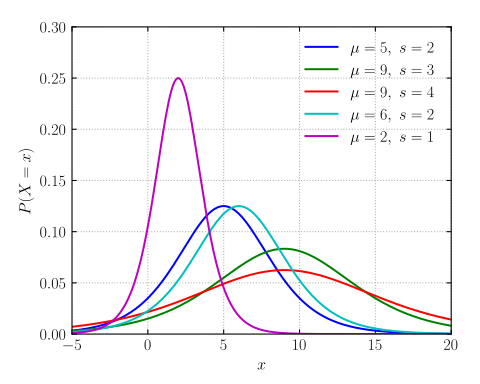
\includegraphics[width=1\textwidth]{LogisticProbDens}
                \caption{Logistic probability density functions AKA logistic distributions}
                \label{subfig: logistic prob distribution}
            \end{minipage}
            \hfill
            \begin{minipage}[t]{0.49\textwidth}
                \centering
                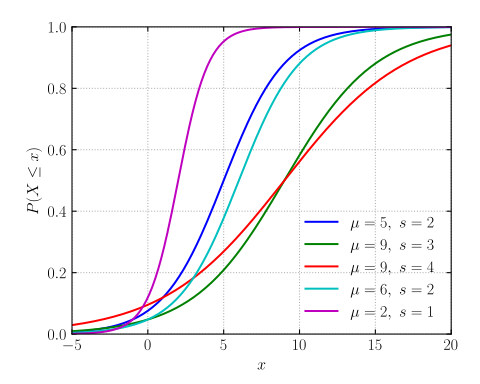
\includegraphics[width=1\textwidth]{LogisticCumDist}
                \caption{Logistic cumulative distributions AKA logistic functions}
                \label{subfig: logistic CDF}
            \end{minipage}
            \caption{Logistic distribution and function}
            \label{fig: logDistFunc}
        \end{figure}

        \begin{figure}[h]
          \caption{Logistic regression models are also called logit models,
          while probit regression models are also called probit models. Logit
          models are used to model Logistic distribution while probit models are
          used to model the cumulative standard normal distribution, as already
          said}
          \centering
          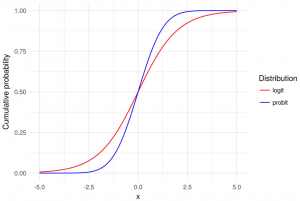
\includegraphics[width=0.55\textwidth]{probitLogitDifference}
          \label{fig: probitvslogit}
          \end{figure}

         \item \textbf{Poisson CDF}: 
        % This link function is rarely used since it performs well in niche
        % cases, such as with a binomial distributions with $\pi \sim \text{
        % Bernoulli }$ (e.g. the number of bacteria on a plate in a dilution
        % bioassay, in which you do not measure the number of bacteria, just
        % whether there are or not). #TODO non so se sia corretto
        Assume that we want to understand if a plate is populated by some
        bacteria. They are distributed accordingly to the $Z_i$ random variable,
        Poisson distributed with parameter $\lambda_i$ ($Z_i \sim \text{ Poisson
        }(\lambda_i)$). $y_i$ takes the following values
        $$
        y_i = 
        \begin{cases}
          0 & \text{ if } z_i = 0 \text{ (absent)} \\
          1 & \text{ if }  z_i > 0 \text{ (present)}
        \end{cases}
        $$
        We would like to describe how $y_i$ changes with time ($x = 0, 1, 2,
        \dots$), therefore we need a function that links $\mu_i$ and $\eta_i$.
        Since we know that 
        $$\eta_i = \log(\lambda_i)$$ and that
        \begin{align*}
        \mu_i 
          &= E[Y_i] \\
          &= 0 \cdot P(Y_i = 0) + 1 \cdot P(Y_i = 1) \\
          &= P(z_i > 0) \\ 
          &= 1 - P(z_i = 0) \\
          &= 1 - e^{-\lambda_i}
        \end{align*}
        we can link $\mu_i$ and $\eta_i$ passing through $\lambda_i$ ($\mu_i
        \leftrightarrow \lambda_i \leftrightarrow \eta_i$). Firstly we rearrange
        the link between $\mu_i$ and $\lambda_i$:
        $$\mu_i = 1 - e^{-\lambda_i} \implies e^{-\lambda_i} = 1 - \mu_i
        \implies \lambda_i = -\log(1 - \mu_i)$$ Then, plugging the $\lambda_i$
        value in the link formula between $\lambda_i$ and $\eta_i$
        ($\log(\lambda_i) = \eta_i$) we get
        $$\eta_i = \log(-\log(1-\mu_i))$$ This link is called
        \textbf{complementary log-log link}.
      \end{enumerate}

    \subsection{Canonical link}
      The logit link is also called \textbf{canonical link} since 
      $$\eta_i = \log\left(\frac{\mu_i}{1-\mu_i}\right) = \theta_i$$ In general
      a canonical link is a function $g$ such that 
      $$\eta_i = g(\mu_i) = \theta_i$$ 
      
      \noindent To put the concept in words, a link function is said to be
      canonical when the relationship between $\mu_i$ and $\nu_i$ is equal to
      that between $\mu_i$ and $\theta_i$. \\
      
      \noindent These link functions have some advantages:
      \begin{itemize}
        \item Clear interpretation of the parameters ($\vec{\beta}$)
        \item Some theoretical reasons (Fisher scoring and iteratively
        reweighted least squares algorithms are equivalent, zero sum residuals)
        \item It follows directly from the EDF formulation of the distribution,
        in fact 
        
        \begin{align*}
          \mu_i &= b^\prime(\theta_i)\\ 
          \theta_i &= (b^\prime)^{-1}(\mu_i)
        \end{align*}

        Since $(b^\prime)^{-1}(\mu_i)$ is the canonical function, it also
        represents the link function.
        

      \end{itemize}
      Despite these advantages the logit link is not always the correct one to
      use.
  
  \section{Residuals in generalized linear models}
    As already seen, a linear model can be express either as:
    $$y_i = \eta_i + \varepsilon_i \text{    (signal (deterministic linear predictor) + noise representation)}$$ Or
    as: 
    $$Y \sim N(\eta_i, \sigma^2)$$

    From the first expression we get the usual definition or residuals in linear
    models:
    $$e_i = y_i - \hat{\eta}_i$$

    Since for generalized linear models we can only use the formulation $Y \sim
    N(\eta_i, \sigma^2)$ (meaning that we cannot simply write the model as value
    plus noise), consequently, we need a new way to define the residuals. There are many
    options, but the most commonly used ones are 
    
    \begin{itemize}
      \item \textbf{Pearson residuals}
      \item \textbf{Deviance residuals}
    \end{itemize}


    \subsection{Pearson residuals}
      Pearson residuals are defined as follows:
      $$r_i^p = \frac{y_i -
      \hat{\mu}_i}{\sqrt{\nicefrac{\hat{Var(y_i)}}{\hat{\phi}}}}$$

      Where $y_i$ represents the observed value of $y$ and $\mu_i$ is the
      predicted mean. If we apply this definition, for instance, to a Poisson
      distribution ($\phi = 1$), we get 
      $$r_i^p = \frac{y_i - \hat{\mu}_i}{\sqrt{\hat{\mu_i}}} \text{ with } y_i
      \in (0, +\infty)$$ Beacause of the interval on which the values of $y_i$
      are defined, the residuals may not be symmetric (in fact, the most
      negative value on the nominator would be $-\hat{\mu_i}$, while instead the
      most positive will be possibly $+\infty$), but the assumption of
      gaussianity is usually satisfied with big values of $\mu$.

    \subsection{Deviance residuals}
      The \textbf{deviance} of an observation $i$ is defined as:
        $$d_i = 2[l_i(y_i; y_i) - l_i(\hat{\mu}_i; y_i)]$$ Where:
      \begin{itemize}
        \item $\hat{\mu}_i = e^{\vec{x}_i^t\hat{\vec{\beta}}}$
        \item $l_i(y_i; y_i)$ is the log-likeihood of the saturated model (most
        fitting non-parametric model, therefore the highest possible likelihood)
        \item $l_i(\hat{\mu}_i; y_i)$ is the log-likelihood of the model using
        the estimated parameters
        \item $d_i \geq 0$, since always $l_i(y_i; y_i) \geq l_i(\hat{\mu}_i; y_i)$
      \end{itemize} \vspace{\baselineskip}
      The overall deviance of the model is defined as the sum of the deviance of
      each observation
      $$\text{deviance } \coloneqq \sum_{i = 1}^n d_i$$ The lower the deviance,
      the closer the model to a perfect fit.
      
      The \textbf{deviance residuals} can be then defined as:
      $$r_i^D = \sqrt{d_i} \cdot \text{sign}(y_i - \hat{\mu_i})\;\; \text{ where
      sign}(y_i - \hat{\mu_i}) = 
      \begin{cases}
        1  & y_i>\hat{\mu_i} \\
        -1 & y_i<\hat{\mu_i} \\
        0  & y_i=\hat{\mu_i}
      \end{cases}
      $$
